\documentclass[conference]{IEEEtran}
\IEEEoverridecommandlockouts

\usepackage{cite}
\usepackage{amsmath,amssymb}
\usepackage{booktabs}
\usepackage{graphicx}
\usepackage{url}
\usepackage{hyperref}
\usepackage{tikz}
\usetikzlibrary{arrows.meta,positioning,shapes.geometric,fit}

\begin{document}

\title{LogShield AI: Canonicalization-Aware BiLSTM Detection of Obfuscated Log4Shell Attempts in Web Request Logs}

\author{%
\begin{tabular}{@{}ccc@{}}
\begin{minipage}[t]{0.31\textwidth}
\centering
Ahmet Faruk Tekeli\\
\textit{Department of Computer Engineering}\\
\textit{Akdeniz University}\\
Antalya, Turkey\\
{\scriptsize\ttfamily 20220808617@ogr.akdeniz.edu.tr}
\end{minipage}
&
\begin{minipage}[t]{0.31\textwidth}
\centering
Ali Berk Ye\c{s}ilduman\\
\textit{Department of Computer Engineering}\\
\textit{Akdeniz University}\\
Antalya, Turkey\\
{\scriptsize\ttfamily 20200808035@ogr.akdeniz.edu.tr}
\end{minipage}
&
\begin{minipage}[t]{0.31\textwidth}
\centering
M\"{u}nevver Nur Topluy\"{u}rek\\
\textit{Department of Computer Engineering}\\
\textit{Akdeniz University}\\
Antalya, Turkey\\
{\scriptsize\ttfamily 20210808067@ogr.akdeniz.edu.tr}
\end{minipage}
\end{tabular}
}

\maketitle

\begin{abstract}
Log4Shell is a critical Apache Log4j vulnerability that enables Remote Code
Execution (RCE) when attacker-controlled log text triggers Java Naming and
Directory Interface (JNDI) lookups. Static signatures are fragile because
attackers can hide the same lookup intent through URL encoding, nested lookup
expressions, environment fallback syntax, Unicode escapes, and token
fragmentation. This paper presents LogShield AI, an obfuscation-aware
Log4Shell detection platform for web request logs. The system combines a
Docker-based traffic laboratory, a provenance-rich dataset pipeline,
canonicalization, a regex baseline, character-level Bidirectional Long
Short-Term Memory (BiLSTM) models, fair evaluation on unseen obfuscation and
adversarial evasion families, live monitoring, an Application Programming
Interface (API), and a dashboard. The goal is not to maximize accuracy on
near-duplicate payloads, but to evaluate whether the detector generalizes to
realistic variants, signature-bypass probes, and hard-negative benign examples.
\end{abstract}

\begin{IEEEkeywords}
Log4Shell, Log4j, Remote Code Execution (RCE), obfuscated payload detection,
Bidirectional Long Short-Term Memory (BiLSTM), web request logs, deep learning
\end{IEEEkeywords}

\section{Introduction}

Log4Shell is a severe Apache Log4j vulnerability that can lead to Remote Code
Execution (RCE) when a logged string is interpreted as a Java Naming and
Directory Interface (JNDI) lookup. A typical payload such as
\texttt{\$\{jndi:ldap://attacker/a\}} can be placed in a HyperText Transfer
Protocol (HTTP) header, path, query parameter, or request body. Bidirectional
Long Short-Term Memory (BiLSTM) models are relevant because the detection
problem is character-sequence oriented: obfuscated variants differ in surface
form but preserve structural character patterns.
CVE-2021-44228 has a Common Vulnerability Scoring System (CVSS) version 3.1
base score of 10.0. We treat it as a supply-chain vulnerability because
vulnerable Log4j versions can be embedded transitively in Java applications
and third-party dependencies.

Figure~\ref{fig:attack_flow} illustrates the Log4Shell attack flow modeled in
this project. The detector is positioned on request-derived log text and
raises an alert when the line contains JNDI lookup evidence after
canonicalization.

\begin{figure}[!t]
\centering
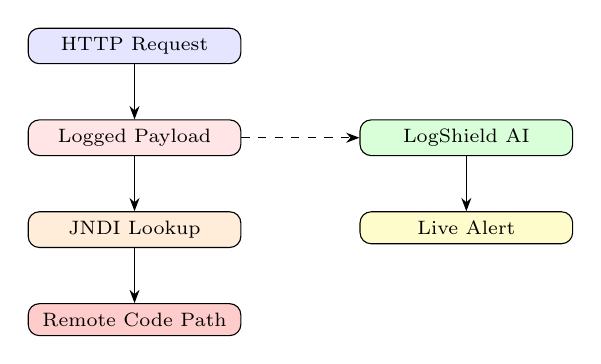
\begin{tikzpicture}[node distance=0.7cm,>=Stealth, every node/.style={font=\scriptsize}]
\node[draw,rounded corners,fill=blue!10,minimum width=2.7cm] (req) {HTTP Request};
\node[draw,rounded corners,fill=red!10,below=of req,minimum width=2.7cm] (log) {Logged Payload};
\node[draw,rounded corners,fill=orange!15,below=of log,minimum width=2.7cm] (jndi) {JNDI Lookup};
\node[draw,rounded corners,fill=red!20,below=of jndi,minimum width=2.7cm] (rce) {Remote Code Path};
\node[draw,rounded corners,fill=green!15,right=1.5cm of log,minimum width=2.7cm] (det) {LogShield AI};
\node[draw,rounded corners,fill=yellow!20,below=of det,minimum width=2.7cm] (alert) {Live Alert};
\draw[->] (req) -- (log);
\draw[->] (log) -- (jndi);
\draw[->] (jndi) -- (rce);
\draw[->,dashed] (log) -- (det);
\draw[->] (det) -- (alert);
\end{tikzpicture}
\caption{Simplified Log4Shell attack flow and defensive log-detection point.}
\label{fig:attack_flow}
\end{figure}

The contributions are: (i) a family-based dataset construction pipeline, (ii)
an obfuscation-aware canonicalizer, (iii) raw and normalized BiLSTM detectors
with a canonicalized regex baseline, and (iv) a reproducible
product prototype with live detection, Application Programming Interface (API)
access, dashboard visualization, and Docker demonstration.

\section{Background and Related Work}

Remote Code Execution (RCE) is a vulnerability class in which an attacker can
cause code execution on a remote system. Java Naming and Directory Interface
(JNDI) is the Java mechanism abused by Log4Shell to resolve attacker-controlled
Lightweight Directory Access Protocol (LDAP), Remote Method Invocation (RMI),
Domain Name System (DNS), or Lightweight Directory Access Protocol Secure
(LDAPS) references. Apache, the Cybersecurity and Infrastructure Security
Agency (CISA), the National Institute of Standards and Technology (NIST),
Microsoft, Cloudflare, and other organizations published detection and
mitigation guidance for this vulnerability family~\cite{apache_security,cisa_advisory,nvd,microsoft_guidance,cloudflare_payloads}.

Signature-based detection is fast but brittle. Attackers can split strings
with \texttt{\$\{lower:...\}}, \texttt{\$\{upper:...\}},
\texttt{\$\{env:NAME:-x\}}, and default-value fragments such as
\texttt{\$\{::-j\}}. Honeypot and measurement work shows that Log4Shell
scanning and exploitation attempts appeared quickly and continued after the
initial disclosure~\cite{honeynet_data,race_vulnerable,greedybear_docs}.

Traditional Web Application Firewalls (WAFs) and Intrusion Detection Systems
(IDSs) rely on signature rules similar to the regex baseline used in this
work. Snort and Suricata community rulesets added Log4Shell detection
shortly after disclosure, but these rules face the same obfuscation-bypass
pressure demonstrated in the adversarial evasion results of this
study~\cite{mirsky2023}. Machine learning approaches for network intrusion
detection, surveyed by Ring~et~al.~\cite{ring2019}, often use flow-level or
packet-level features rather than request-log text, making direct comparison
difficult. Recent work by Ferrag~et~al.~\cite{ferrag2020} showed that deep
learning models outperform traditional approaches on cybersecurity text
classification when trained on representative datasets.

Sequence models such as Long Short-Term Memory (LSTM) networks and
Bidirectional Long Short-Term Memory (BiLSTM) networks are useful when the
input is a raw character sequence rather than a clean token stream
\cite{hochreiter1997,graves2013}. Saxe and Berlin~\cite{saxe2017}
demonstrated that character-level convolutional models can detect malicious
URLs and file paths without hand-crafted features; this work extends the
character-level approach to obfuscated Log4Shell payloads with a BiLSTM
backbone. Attention mechanisms, originally proposed for neural machine
translation by Bahdanau~et~al.~\cite{bahdanau2015}, allow the model to
focus on the most suspicious character subsequences in a log line.

Unlike prior Log4Shell detection efforts that report accuracy on
near-duplicate test sets, this work evaluates on held-out obfuscation
families, adversarial evasion probes, hard-negative false-positive stress,
and frozen out-of-distribution splits. The KDD Cup 99 dataset analysis by
Tavallaee~et~al.~\cite{kdd_analysis} demonstrated the importance of
removing duplicate records for fair evaluation; the family-based split
strategy used here follows a similar principle.

\section{Threat Model and Problem Definition}

In this section, HyperText Transfer Protocol (HTTP) logs are the only assumed
input. The attacker controls one or more request fields and may obfuscate a
Java Naming and Directory Interface (JNDI) lookup using encodings or Log4j
lookup syntax. The defender can collect logs and run detection, but the system
does not inspect process execution, bytecode loading, or outbound callbacks.

The binary classification task is to assign each log line a benign or
malicious label, then map the final risk score into benign, suspicious, or
malicious product states. This limitation is important: the system detects
visible exploitation attempts, not successful exploitation.

\section{Dataset Construction}

The dataset construction stage uses HyperText Transfer Protocol (HTTP)
request-like logs with a shared schema that records provenance, normalized
text, label, attack family, obfuscation type, affected field, split, and risk
level. The final corpus contains 4,922 rows: 2,020 training rows, 422
validation rows, and 2,480 evaluation rows across standard, unseen,
adversarial, hard-negative, external, blind, and frozen stress-test files.
Benign rows include normal request paths, user agents, search strings,
documentation-like examples, suspicious but non-executing tokens, and public
Apache access logs. Malicious rows preserve Log4Shell lookup semantics while
varying protocol, request field, encoding, and obfuscation family. The section
uses Uniform Resource Locator (URL), Java Naming and Directory Interface
(JNDI), and Packet Capture (PCAP) terminology for the payload and external
validation sources. Table~\ref{tab:sources} summarizes the dataset sources and
their roles. The table is created by us from the repository pipeline rather
than copied from external work.

\begin{table}[!t]
\caption{Dataset sources and their evaluation roles.}
\label{tab:sources}
\centering
\resizebox{\columnwidth}{!}{%
\begin{tabular}{lll}
\toprule
Source & Role & Split Use \\
\midrule
Synthetic payloads & Controlled malicious variants & Train/Validation/Test \\
Benign logs & Normal web behavior & Train/Validation/Test \\
Apache-format benign logs & Access-log format hardening & Train/Validation/Test \\
Hard negatives & Suspicious benign text & Train/Test \\
Honeypot feeds & Real-derived malicious signal & External \\
PCAP-derived HTTP & Packet-capture validation & External \\
Splunk attack data & Access-log style validation & External \\
Elastic Apache logs & Benign external false-positive check & External \\
Payload corpora & Obfuscation taxonomy expansion & Unseen Test \\
CuratedIntel indicators & Callback context metadata & Metadata Only \\
\bottomrule
\end{tabular}
}
\end{table}

Table~\ref{tab:taxonomy} explains the obfuscation taxonomy used to prevent
near-duplicate train/test leakage. Training includes plain payloads, common
protocol variants, simple URL encoding, case manipulation, and a limited set
of evasion examples. The unseen test set contains nested lookup, environment
fallback, fragmented token, double URL encoding, Unicode escape, and
mixed-separator variants. A dedicated adversarial evasion test set contains
zero-width characters, Unicode homoglyphs, HTML entities, triple URL encoding,
semantic lookup reconstruction, lookup-character concatenation, context
embedding, whitespace or comment insertion, and simulated field splitting.

\begin{table}[!t]
\caption{Obfuscation families used for family-based evaluation.}
\label{tab:taxonomy}
\centering
\begin{tabular}{ll}
\toprule
Family & Example Intent \\
\midrule
Plain JNDI & Direct lookup syntax \\
URL encoded & Encoded braces and separators \\
Nested lookup & Lower/upper expression composition \\
Environment fallback & Default-value character recovery \\
Fragmented tokens & Split JNDI characters \\
Unicode escape & Escaped character bytes \\
Adversarial evasion & Signature-bypass probe syntax \\
Hard negative & Benign suspicious text \\
\bottomrule
\end{tabular}
\end{table}

\section{Proposed Detection Pipeline}

The proposed pipeline receives request logs, canonicalizes them, builds
character-level features, compares signature and Bidirectional Long Short-Term
Memory (BiLSTM) model outputs, and emits a risk score through the Application
Programming Interface (API) and dashboard. Figure~\ref{fig:pipeline} shows the
complete engineering workflow from Docker laboratory traffic to reporting.

\begin{figure}[!t]
\centering
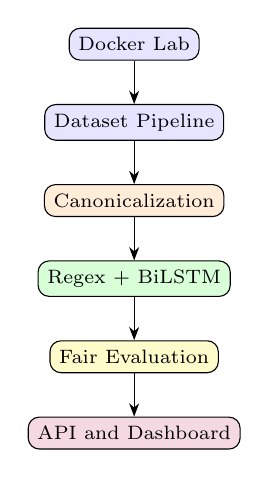
\begin{tikzpicture}[node distance=0.55cm,>=Stealth, every node/.style={font=\scriptsize}]
\node[draw,rounded corners,fill=blue!10] (lab) {Docker Lab};
\node[draw,rounded corners,fill=blue!10,below=of lab] (data) {Dataset Pipeline};
\node[draw,rounded corners,fill=orange!15,below=of data] (canon) {Canonicalization};
\node[draw,rounded corners,fill=green!15,below=of canon] (model) {Regex + BiLSTM};
\node[draw,rounded corners,fill=yellow!20,below=of model] (eval) {Fair Evaluation};
\node[draw,rounded corners,fill=purple!15,below=of eval] (live) {API and Dashboard};
\draw[->] (lab) -- (data);
\draw[->] (data) -- (canon);
\draw[->] (canon) -- (model);
\draw[->] (model) -- (eval);
\draw[->] (eval) -- (live);
\end{tikzpicture}
\caption{End-to-end Log4Shell detection pipeline used in the proposed system.}
\label{fig:pipeline}
\end{figure}

The canonicalization engine performs repeated Uniform Resource Locator (URL)
decoding, HyperText Markup Language (HTML) entity decoding, Unicode escape decoding, lowercase
normalization, lookup expression resolution, and fragmented token
reconstruction. Figure~\ref{fig:canonicalization} illustrates how an
obfuscated payload is mapped to a simpler canonical form before detection.

\begin{figure}[!t]
\centering
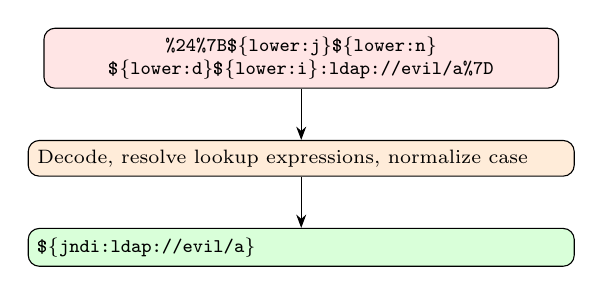
\begin{tikzpicture}[node distance=0.65cm,>=Stealth, every node/.style={font=\scriptsize}]
\node[draw,rounded corners,fill=red!10,text width=6.3cm,align=center] (raw)
{\texttt{\%24\%7B\$\{lower:j\}\$\{lower:n\}}\\
\texttt{\$\{lower:d\}\$\{lower:i\}:ldap://evil/a\%7D}};
\node[draw,rounded corners,fill=orange!15,below=of raw,text width=6.7cm] (steps) {Decode, resolve lookup expressions, normalize case};
\node[draw,rounded corners,fill=green!15,below=of steps,text width=6.7cm] (norm) {\texttt{\$\{jndi:ldap://evil/a\}}};
\draw[->] (raw) -- (steps);
\draw[->] (steps) -- (norm);
\end{tikzpicture}
\caption{Canonicalization example for an encoded and nested Log4Shell payload.}
\label{fig:canonicalization}
\end{figure}

\section{Model Architecture}

The Long Short-Term Memory (LSTM) component receives padded character indices.
The Bidirectional Long Short-Term Memory (BiLSTM) variant reads the sequence in
both directions, making it suitable for payloads where suspicious tokens can
appear in paths, headers, or body fields. Figure~\ref{fig:model} shows the
model architecture used by the main detector.

\begin{figure}[!t]
\centering
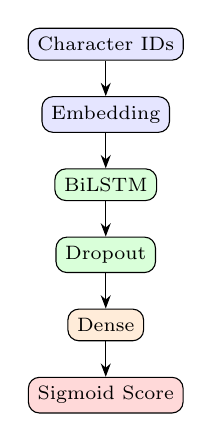
\begin{tikzpicture}[node distance=0.45cm,>=Stealth, every node/.style={font=\scriptsize}]
\node[draw,rounded corners,fill=blue!10] (inp) {Character IDs};
\node[draw,rounded corners,fill=blue!10,below=of inp] (emb) {Embedding};
\node[draw,rounded corners,fill=green!15,below=of emb] (bi1) {BiLSTM};
\node[draw,rounded corners,fill=green!15,below=of bi1] (drop) {Dropout};
\node[draw,rounded corners,fill=orange!15,below=of drop] (dense) {Dense};
\node[draw,rounded corners,fill=red!15,below=of dense] (out) {Sigmoid Score};
\draw[->] (inp) -- (emb);
\draw[->] (emb) -- (bi1);
\draw[->] (bi1) -- (drop);
\draw[->] (drop) -- (dense);
\draw[->] (dense) -- (out);
\end{tikzpicture}
\caption{Character-level BiLSTM architecture for Log4Shell request-log classification.}
\label{fig:model}
\end{figure}

The implemented detector compares five model families: canonicalized regex
baseline, raw BiLSTM, normalized BiLSTM, BiLSTM with attention, and BiLSTM with
canonical signals. Table~\ref{tab:hyperparams} lists the training
hyperparameters and architecture dimensions.

\begin{table}[!t]
\caption{Training hyperparameters and architecture configuration.}
\label{tab:hyperparams}
\centering
\begin{tabular}{ll}
\toprule
Parameter & Value \\
\midrule
Character vocabulary size & 93 \\
Max sequence length & 512 \\
Embedding dimension & 64 \\
BiLSTM layer 1 units & 128 (per direction) \\
BiLSTM layer 2 units & 64 (per direction) \\
Attention BiLSTM units & 96 (per direction) \\
Dense hidden units & 64 (base) / 96+32 (attention) \\
Dropout rate & 0.30 (base) / 0.20 (attention) \\
Optimizer & Adam \\
Learning rate & $1 \times 10^{-3}$ (base) / $8 \times 10^{-4}$ (attention) \\
Loss function & Binary cross-entropy \\
Class weighting & Balanced (sklearn) \\
Epochs & 8 (early stopping patience 3) \\
Batch size & 64 \\
Canonical signal features & 13 (signal variant only) \\
Training rows & 2,020 \\
Validation rows & 422 \\
\bottomrule
\end{tabular}
\end{table}

\section{Experimental Setup}

The evaluation reports accuracy, precision, recall, F1-score, Receiver
Operating Characteristic Area Under the Curve (ROC-AUC), Precision-Recall Area
Under the Curve (PR-AUC), false-positive rate (FPR), false-negative rate
(FNR), latency, and throughput. Packet Capture (PCAP) rows are used only for
external validation. Evaluation thresholds are calibrated on the validation
set. Table~\ref{tab:evaluation} lists the required test sets.
The test design separates standard variants, unseen obfuscation, adversarial
evasion probes, hard negatives, external validation, and blind manual examples.

\begin{table}[!t]
\caption{Evaluation sets used by the final comparison script.}
\label{tab:evaluation}
\centering
\resizebox{\columnwidth}{!}{%
\begin{tabular}{lrl}
\toprule
Test Set & Rows & Purpose \\
\midrule
test.csv & 282 & Standard held-out examples \\
unseen\_obfuscation\_test.csv & 589 & New obfuscation families \\
adversarial\_evasion\_test.csv & 792 & Signature-bypass probes \\
hard\_negative\_test.csv & 180 & False-positive resistance \\
external\_greedybear\_test.csv & 60 & Honeypot-derived validation \\
external\_splunk\_test.csv & 1 & Access-log style validation \\
external\_foxit\_pcap\_test.csv & 4 & PCAP-derived validation \\
external\_benign\_web\_test.csv & 200 & Public benign web-log validation \\
blind\_manual\_test.csv & 84 & Presentation sanity check \\
ood\_stress\_test.csv & 288 & Frozen generalization stress test \\
\bottomrule
\end{tabular}
}
\end{table}

\section{Results and Discussion}

The repository generates the final model comparison in
\texttt{results/final\_comparison.csv}. Table~\ref{tab:model_comparison}
summarizes the main Bidirectional Long Short-Term Memory (BiLSTM) detector
rows for the standard test set, unseen
obfuscation set, adversarial evasion set, frozen out-of-distribution (OOD)
stress set, and hard-negative set. The false-positive rate (FPR) columns make
hard-negative false positives, evasion recall, and generalization behavior
visible. Single-class external and evasion-only sets
report undefined Receiver Operating Characteristic Area Under the Curve
(ROC-AUC) and Precision-Recall Area Under the Curve (PR-AUC) values as
Not a Number (\texttt{NaN}). The first three F1-score columns are the original
benchmark splits; the OOD columns are the frozen post-training stress-test
results.

\begin{table}[!t]
\caption{Original benchmark and frozen OOD stress-test summary.}
\label{tab:model_comparison}
\centering
\resizebox{\columnwidth}{!}{%
\begin{tabular}{lcccccc}
\toprule
Model & Standard F1 & Unseen F1 & Evasion F1 & OOD F1 & OOD FPR & Hard FPR \\
\midrule
Regex Baseline & 1.000 & 1.000 & 0.842 & 0.200 & 0.500 & 0.478 \\
Raw BiLSTM & 1.000 & 1.000 & 0.952 & 0.783 & 0.167 & 0.000 \\
Normalized BiLSTM & 1.000 & 1.000 & 0.952 & 0.545 & 0.333 & 0.000 \\
BiLSTM + Attention & 1.000 & 1.000 & 1.000 & 0.468 & 0.000 & 0.000 \\
BiLSTM + Signal & 1.000 & 1.000 & 0.952 & 0.564 & 0.167 & 0.000 \\
\bottomrule
\end{tabular}
}
\end{table}

Table~\ref{tab:raw_counts} reports the baseline regex F1-score, the final Raw
BiLSTM F1-score, true positives (TP), true negatives (TN), false positives
(FP), and false negatives (FN) on every generated test split. The confusion
counts belong to the Raw BiLSTM model. Single-class rows are expected for
malicious-only or benign-only supplementary test files, and benign-only F1
values are less informative than the false-positive counts.

\begin{table}[!t]
\caption{Final regex and Raw BiLSTM results for every generated test split.}
\label{tab:raw_counts}
\centering
\resizebox{\columnwidth}{!}{%
\begin{tabular}{lrrrrrr}
\toprule
Test Split & Regex F1 & Raw F1 & TP & TN & FP & FN \\
\midrule
Standard test & 1.000 & 1.000 & 72 & 210 & 0 & 0 \\
Unseen obfuscation & 1.000 & 1.000 & 589 & 0 & 0 & 0 \\
Adversarial evasion & 0.842 & 0.952 & 720 & 0 & 0 & 72 \\
Hard negative & 0.000 & 0.000 & 0 & 180 & 0 & 0 \\
Honeynet external & 1.000 & 1.000 & 60 & 0 & 0 & 0 \\
Splunk external & 1.000 & 1.000 & 1 & 0 & 0 & 0 \\
Fox-IT PCAP external & 1.000 & 1.000 & 4 & 0 & 0 & 0 \\
External benign web & 0.000 & 0.000 & 0 & 200 & 0 & 0 \\
Blind manual & 0.364 & 1.000 & 4 & 80 & 0 & 0 \\
Frozen OOD stress & 0.200 & 0.783 & 108 & 120 & 24 & 36 \\
\bottomrule
\end{tabular}
}
\end{table}

The adversarial evasion split directly addresses the signature-bypass question.
The canonicalized regex baseline detects 576 of 792 evasion payloads (recall
0.727, F1-score 0.842), but still misses 216 held-out evasion payloads. In the
same run, raw, normalized, and signal BiLSTM variants detect 720 of 792
examples, while BiLSTM with attention detects all 792 adversarial evasion
examples. This result shows that the learned detector adds value beyond the
regex baseline, while the canonicalized regex still remains useful for fast
known-pattern coverage.
Because the evasion set contains only malicious examples, Receiver Operating
Characteristic Area Under the Curve (ROC-AUC) and Precision-Recall Area Under
the Curve (PR-AUC) are intentionally undefined for that split.

To address the risk that perfect neural scores reflect an overly easy
synthetic benchmark, the final run also includes a frozen out-of-distribution
(OOD) stress split. This split is generated after training and is not used for
training, validation, regex tuning, threshold calibration, or model selection.
It contains 144 new malicious evasion probes and 144 benign display-only
payload examples. On this stress split, the regex baseline reaches only
0.167 recall and 0.200 F1-score. After hard-negative and external-format
benign training, Raw BiLSTM provides the best final balance with 0.750 recall,
0.783 F1-score, and 0.167 false-positive rate. The normalized BiLSTM reaches
0.545 OOD F1-score, and the signal-augmented variant reaches 0.564 OOD
F1-score, showing that extra canonical features do not automatically improve
generalization. BiLSTM with attention provides the lowest OOD false-positive
rate (0.000), but with lower malicious recall (0.306). This result is reported
as a limitation: false-positive reduction introduces a precision/recall
tradeoff on frozen OOD probes.

The ablation study compares raw text, normalized text, canonical signals,
regex-only detection, and BiLSTM-only detection. Error
analysis records model-specific false positives and false negatives with their
source, normalized form, score, threshold, obfuscation type, and explanation.
The held-out hard-negative test is retained as a direct false-positive check:
the neural detectors produce a hard-negative false-positive rate of 0.000,
while the regex baseline flags 86 of 180 benign hard-negative examples.
Supplementary external validation was expanded to 265 rows: 65 fetched
malicious rows from Honeynet, Splunk, and Fox-IT sources plus 200 public benign
Apache access-log rows from Elastic examples. Raw BiLSTM and BiLSTM with
attention detect all 65 malicious external rows and all neural detectors
produce 0 false positives on the 200 benign external Apache rows. These
external rows are used as supplementary validation rather than population-level
performance estimates.

\section{Live Detection Demo}

The Application Programming Interface (API), Streamlit dashboard, file monitor,
and Docker Compose demo show the system as an end-to-end product prototype.
Figure~\ref{fig:live} explains the live demonstration workflow used in the
presentation.

\begin{figure}[!t]
\centering
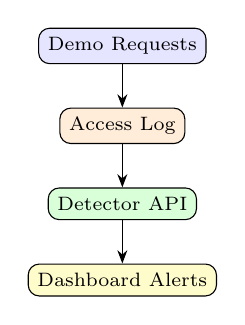
\begin{tikzpicture}[node distance=0.55cm,>=Stealth, every node/.style={font=\scriptsize}]
\node[draw,rounded corners,fill=blue!10] (gen) {Demo Requests};
\node[draw,rounded corners,fill=orange!15,below=of gen] (logs) {Access Log};
\node[draw,rounded corners,fill=green!15,below=of logs] (api) {Detector API};
\node[draw,rounded corners,fill=yellow!20,below=of api] (dash) {Dashboard Alerts};
\draw[->] (gen) -- (logs);
\draw[->] (logs) -- (api);
\draw[->] (api) -- (dash);
\end{tikzpicture}
\caption{Live detection workflow used by the reproducible Docker demonstration.}
\label{fig:live}
\end{figure}

\section{Limitations and Ethical Considerations}

The dataset is mixed-source and partially synthetic. Real-world labeled
HyperText Transfer Protocol (HTTP)
Log4Shell datasets are limited, and some external validation files are
single-class malicious or single-class benign sets. Packet-capture validation
depends on local \texttt{tshark} availability. External validation is therefore
reported as supplementary evidence rather than a population-level estimate. The detector may
miss unknown obfuscation strategies and should support, not replace, patch
management, dependency inventory, egress monitoring, and runtime protections.
The Docker laboratory is defensive and does not include a weaponized exploit
server.

\section{Conclusion}

This paper presented LogShield AI, an obfuscation-resistant Log4Shell detection
platform centered on character-level Bidirectional Long Short-Term Memory
(BiLSTM) modeling. The main engineering result is an end-to-end defensive
pipeline that combines dataset construction, canonicalization, baseline
comparison, fair evaluation, live monitoring, Application Programming
Interface (API) access, dashboard
visualization, and reproducible Docker demonstration.

The key experimental findings are: (i) all neural detectors achieve F1-score
1.000 on the standard test split and complete recall on the reserved
unseen-obfuscation malicious split, while false-positive behavior is
interpreted using hard-negative, blind/manual, external benign, and frozen
out-of-distribution tests; (ii) the BiLSTM with attention variant detects all 792 adversarial evasion
payloads (recall 1.000), whereas the canonicalized regex baseline misses
27.3\% of them; (iii) all neural detectors produce a hard-negative
false-positive rate of 0.000, compared to 0.478 for the regex baseline;
and (iv) the frozen out-of-distribution stress test reveals a
precision/recall tradeoff, with Raw BiLSTM achieving the best balance
(F1-score 0.783) and BiLSTM with attention achieving the lowest
false-positive rate (0.000) at the cost of lower recall.

The ablation study shows that explicit canonical signal features do not
automatically improve generalization, and that normalization can reduce
robustness on certain out-of-distribution patterns. These negative results
are reported to avoid overstating the contribution of individual pipeline
components.

Future work includes: (i) replacing the BiLSTM backbone with a
pre-trained Transformer encoder such as a character-level BERT variant to
improve contextual representation; (ii) ensemble scoring that combines
regex speed with neural recall; (iii) expanding the training set with
real-world honeypot traffic from additional deployment sites;
(iv) adversarial training with generated evasion samples to close the
frozen out-of-distribution recall gap; and (v) extending the detector
to other log-injectable vulnerabilities beyond Log4Shell.

\begin{thebibliography}{00}
\bibitem{apache_security} Apache Logging Services, ``Apache Log4j Security Vulnerabilities,'' \url{https://logging.apache.org/log4j/2.x/security}.
\bibitem{cisa_advisory} CISA, FBI, NSA, and international partners, ``Mitigating Log4Shell and Other Log4j-Related Vulnerabilities,'' Joint Cybersecurity Advisory AA21-356A, 2021.
\bibitem{nvd} NIST National Vulnerability Database, ``CVE-2021-44228 Detail,'' \url{https://nvd.nist.gov/vuln/detail/CVE-2021-44228}.
\bibitem{microsoft_guidance} Microsoft, ``Guidance for preventing, detecting, and hunting for exploitation of the Log4j 2 vulnerability,'' 2021.
\bibitem{cloudflare_payloads} Cloudflare, ``Actual CVE-2021-44228 payloads captured in the wild,'' 2021.
\bibitem{honeynet_data} Honeynet Project, ``log4shell-data,'' \url{https://github.com/honeynet/log4shell-data}.
\bibitem{greedybear_docs} The Honeynet Project, ``GreedyBear Usage Documentation,'' \url{https://greedybear-docs.readthedocs.io/en/latest/Usage.html}.
\bibitem{foxit_pcaps} Fox-IT, ``Log4Shell PCAPS and Network Coverage,'' \url{https://github.com/fox-it/log4shell-pcaps}.
\bibitem{splunk_attack_data} Splunk, ``Log4Shell attack data,'' \url{https://research.splunk.com/attack_data/987c92c7-defa-4a3a-baf4-3973501aec8c/}.
\bibitem{payloadsallthethings} PayloadsAllTheThings, ``CVE-2021-44228 Log4Shell,'' \url{https://swisskyrepo.github.io/PayloadsAllTheThings/CVE%20Exploits/Log4Shell/}.
\bibitem{curatedintel} Curated Intelligence, ``Log4Shell IOCs,'' \url{https://github.com/curated-intel/Log4Shell-IOCs}.
\bibitem{hochreiter1997} S. Hochreiter and J. Schmidhuber, ``Long Short-Term Memory,'' \textit{Neural Computation}, vol. 9, no. 8, pp. 1735--1780, 1997.
\bibitem{graves2013} A. Graves, A. Mohamed, and G. Hinton, ``Speech recognition with deep recurrent neural networks,'' in \textit{Proc. IEEE ICASSP}, 2013, pp. 6645--6649.
\bibitem{saxe2017} J. Saxe and K. Berlin, ``eXpose: A character-level convolutional neural network with embeddings for detecting malicious URLs, file paths and registry keys,'' arXiv:1702.08568, 2017.
\bibitem{ring2019} M. Ring, S. Wunderlich, D. Scheuring, D. Landes, and A. Hotho, ``A survey of network-based intrusion detection data sets,'' \textit{Computers \& Security}, vol. 86, pp. 147--167, 2019.
\bibitem{kdd_analysis} M. Tavallaee, E. Bagheri, W. Lu, and A. A. Ghorbani, ``A detailed analysis of the KDD CUP 99 data set,'' in \textit{Proc. IEEE CISDA}, 2009, pp. 1--6.
\bibitem{race_vulnerable} J. A. Ruohonen, ``The race to the vulnerable: Measuring the Log4j shell incident,'' arXiv:2205.02544, 2022.
\bibitem{mirsky2023} Y. Mirsky, T. Doitshman, Y. Elovici, and A. Shabtai, ``Kitsune: An ensemble of autoencoders for online network intrusion detection,'' in \textit{Proc. NDSS}, 2018, pp. 1--15.
\bibitem{ferrag2020} M. A. Ferrag, L. Maglaras, S. Moschoyiannis, and H. Janicke, ``Deep learning for cyber security intrusion detection: Approaches, datasets, and comparative study,'' \textit{Journal of Information Security and Applications}, vol. 50, 102419, 2020.
\bibitem{bahdanau2015} D. Bahdanau, K. Cho, and Y. Bengio, ``Neural machine translation by jointly learning to align and translate,'' in \textit{Proc. ICLR}, 2015.
\end{thebibliography}

\end{document}
